\documentclass{homework}
    
\author{Germán Braun}
\class{Aprendizaje Automático}
\date{\today}
\title{Laboratorio 1}
\address{}

\graphicspath{{./media/}}

\begin{document} \maketitle

\section*{Introducción al Aprendizaje Automático}

\question Dar al menos 2 aplicaciones para las cuales el uso aprendizaje automático es apropiado y 2 en las que no. Justifique.

\question Seleccione al menos 1 de los ejemplos del ejercicio anterior y defina el problema de aprendizaje asociado, dando una tarea ($T$), la medida de performance ($P$), y conjunto de entrenamiento ($E$) 

\question Dada la siguiente matriz de confusión de un modelo clasificador de spams:

\begin{figure}[h!]
    \centering
    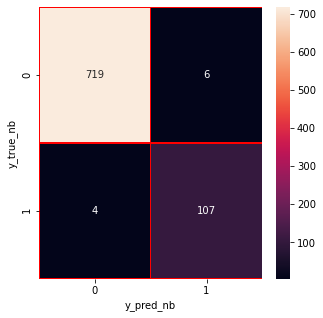
\includegraphics[width=0.5\linewidth]{mconf.png}
    \caption{Matriz de Confusión}\label{fig:matriz}
\end{figure}

\begin{enumerate}
    \item calcular precisión, recall, especificidad y exactitud
    \item explique que sucede en un escenario de alta precisión pero bajo recall
    \item de algún ejemplo en el cual la métrica de especificidad tenga relevancia 
\end{enumerate}

\question Explique en que casos es útil el \textbf{F-score}


\question Dada el gráfico \ref{fig:roc} visto en la clase, explique las curvas allí presentes y agregue dos algoritmos que tengan mayor rendimiento (TPR) que los anteriores. 

\begin{figure}[h!]
    \centering
    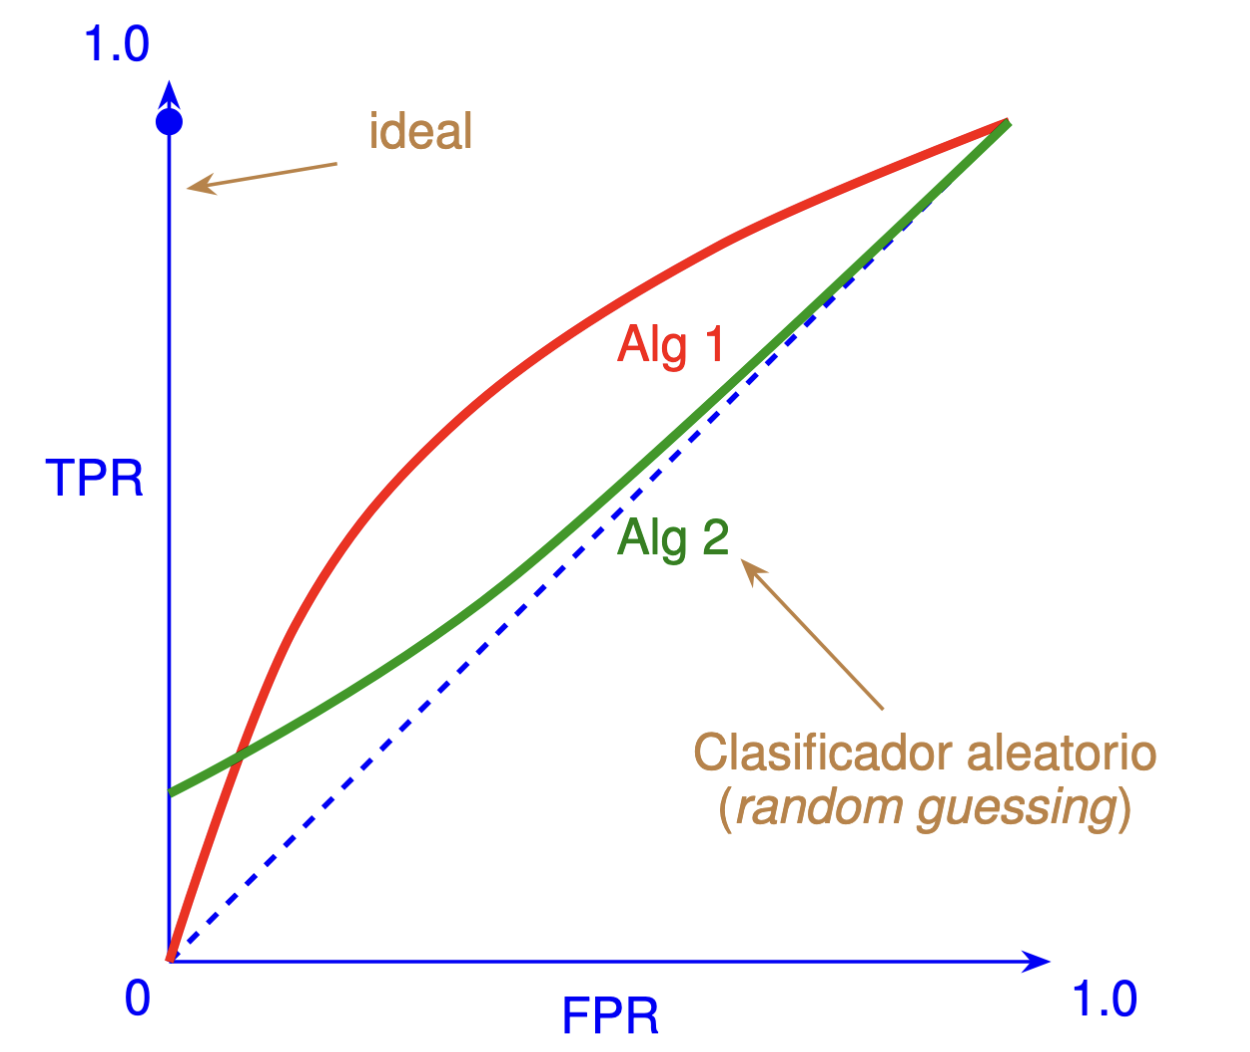
\includegraphics[width=0.5\linewidth]{ROC.png}
    \caption{Curva ROC}\label{fig:roc}
\end{figure}

\question Explique los siguientes conceptos y ejemplifique:

\begin{enumerate}
    \item underfitting
    \item overfitting
    \item relación de estos conceptos con sesgo y varianza
    \item Qué puede concluir del gráfico \ref{fig:bias} sobre la complejidad óptima de un modelo\footnote{imagen de \url{https://scott.fortmann-roe.com/docs/BiasVariance.html}}? 
\end{enumerate}

\begin{figure}[h!]
    \centering
    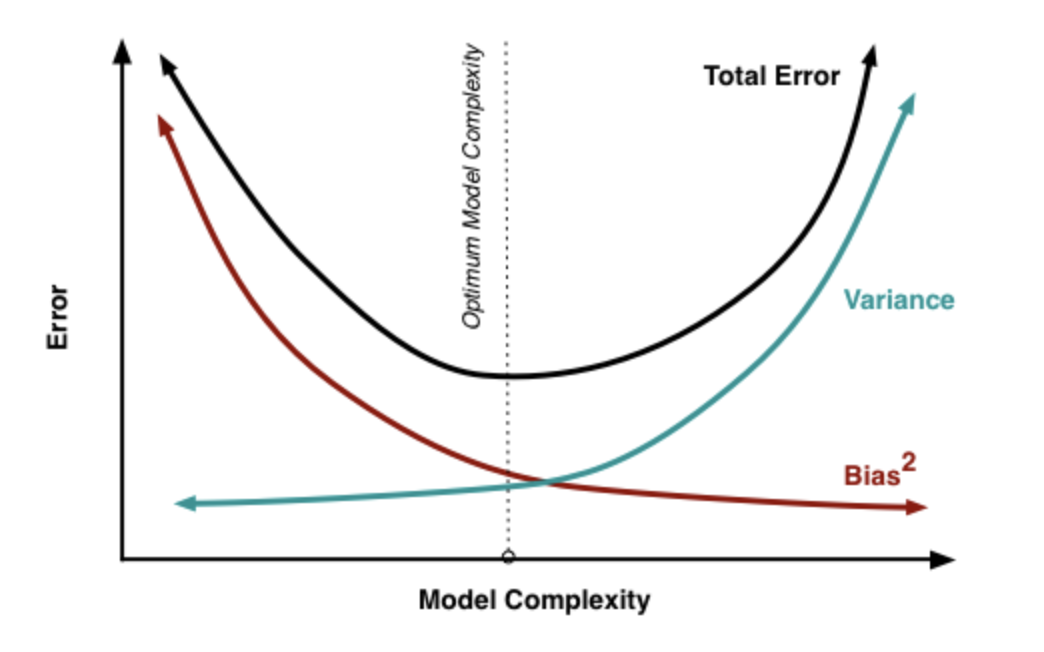
\includegraphics[width=0.55\linewidth]{bias-variance.png}
    \caption{Sesgo y Varianza}\label{fig:bias}
\end{figure}


\newpage
\section*{Aspectos Éticos}

\question Enumere al menos 2 sesgos que ocurren/podrían ocurrir al utilizar IA

\question Explique por qué la IA basada en Aprendizaje Automático y, en particular las Generativas, heredan sesgos de la sociedad.

\end{document}
